\documentclass[aspectratio=169]{beamer}
% --- PACKAGES ET CONFIGURATION ---
\usepackage[english]{babel}
\usepackage[T1]{fontenc}
\usepackage{amsmath, amssymb, bm, mathtools}
\usepackage{booktabs, xcolor, colortbl}
\usepackage{tcolorbox}
\usepackage{graphicx}
\usepackage{comment}
\usepackage{tikz}
\usetikzlibrary{decorations.pathreplacing, positioning}
\tcbuselibrary{skins}

% --- DESIGN ET COULEURS (template original) ---
\definecolor{primary}{RGB}{15, 45, 80}
\definecolor{secondary}{RGB}{0, 150, 136}
\definecolor{bglight}{RGB}{245, 247, 250}
\definecolor{softblue}{RGB}{235,238,245}
\usetheme{Madrid}
\usecolortheme{whale}
\setbeamercolor{structure}{fg=primary}
\setbeamercolor{title}{fg=white, bg=primary}
\setbeamercolor{block title}{bg=primary, fg=white}
\setbeamercolor{block body}{bg=primary!5, fg=black}
\setbeamercolor{palette primary}{bg=primary, fg=white}
\setbeamercolor{palette secondary}{bg=secondary, fg=white}
\setbeamertemplate{navigation symbols}{}
\setbeamertemplate{items}[circle]
\setbeamertemplate{headline}{}

% --- COMMANDES PERSO ---
\newcommand{\R}{\mathbb{R}}
\newcommand{\E}{\mathbb{E}}
\newcommand{\loss}{\mathcal{L}}

% --- CLEAN CARDS (replace the default beamer blocks on busy slides) ---
% #1 = accent color, #2 = equal-height group name
\newtcolorbox{qbox}[2]{%
  enhanced, nobeforeafter,
  colback=bglight, colframe=#1,
  boxrule=0pt, leftrule=3.5pt, arc=3pt,
  left=8pt, right=7pt, top=8pt, bottom=8pt,
  equal height group=#2,
  before upper={\setlength{\parskip}{0pt}}
}
% numbered badge + title:  \cardhead{accent}{number}{title}
\newcommand{\cardhead}[3]{%
  {\tikz[baseline=-0.6ex]\node[circle, fill=#1, text=white,
        font=\scriptsize\bfseries, inner sep=1.7pt, minimum size=4.5mm]{#2};}%
  \hspace{3pt}\textbf{\color{#1}#3}\par\vspace{5pt}}
% simple title (no number)
\newcommand{\cardtitle}[2]{\textbf{\color{#1}#2}\par\vspace{5pt}}
% compact item list inside cards
\newcommand{\qitem}[1]{\textcolor{secondary}{\footnotesize$\bullet$}\hspace{4pt}#1\par\vspace{3pt}}

\title[Hack the World(s)]{Hack The World(s)}
\author[Azéma, Kheng, Le Pendeven]{Azéma Tanguy, Kheng Augustin, Le Pendeven Théo}
\institute[]{}
\date{\today}

\begin{document}

% ---------------------------------------------------------------
% TITLE
% ---------------------------------------------------------------
\frame{\titlepage}

% ---------------------------------------------------------------
% AGENDA
% ---------------------------------------------------------------
\begin{frame}{Agenda}
  \tableofcontents
\end{frame}

% =================================================================
% SECTION 1 — WHAT YOU HAVE & WHAT WE EXPECT
% =================================================================
\section{What You Have \& What We Expect}

% --- 1a. Data overview (two types) ---
\begin{frame}{The Data You Will Work With}
  \begin{center}
    \small Two main types of data are available for the challenge.
  \end{center}
  \vspace{0.3cm}

  \begin{columns}[T]
    \begin{column}{0.47\textwidth}
      \begin{block}{1 — Datasets we provide}
        Ready-to-use datasets from different domains:
        \begin{itemize}
          \item \textbf{Neuroscience} — neural recordings
          \item \textbf{Audio} — audio/speech files
          \item \textbf{Physion} — physical reasoning / object dynamics
        \end{itemize}
        \vspace{0.1cm}
        \footnotesize\itshape Just load them and start training.
      \end{block}
    \end{column}

    \begin{column}{0.47\textwidth}
      \begin{block}{2 — Data you generate}
        Datasets you build yourselves, following our example:
        \begin{itemize}
        \item \textbf{Two rooms}
          \item \textbf{Maze} — our reference example (see Section 2)
          \item Serves as a \textbf{pipeline} you can reuse and adapt
        \end{itemize}
        \vspace{0.1cm}
        \footnotesize\itshape Full generation code is provided as a starting point.
      \end{block}
    \end{column}
  \end{columns}

  \vspace{0.3cm}
  \begin{center}
    \small You may use one type, the other, or both.
  \end{center}
\end{frame}

% --- 1b. The model / reference pipeline ---
\begin{frame}{The Model — A JEPA Baseline}
  \begin{center}
    \resizebox{0.82\textwidth}{!}{%
    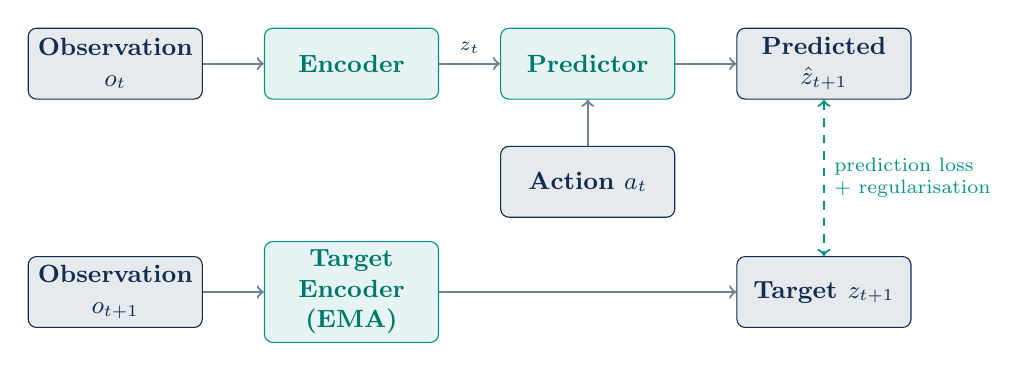
\begin{tikzpicture}[
      every node/.style={font=\small},
      nd/.style={draw=primary, fill=primary!10, rounded corners=3pt,
                 text width=2cm, minimum height=0.9cm,
                 align=center, font=\small\bfseries, text=primary, inner sep=3pt},
      nd2/.style={draw=secondary, fill=secondary!10, rounded corners=3pt,
                  text width=2cm, minimum height=0.9cm,
                  align=center, font=\small\bfseries, text=secondary!80!black, inner sep=3pt},
      ar/.style={->, thick, color=primary!60}
    ]
      % top: context flow
      \node[nd]  (obs)  at (0,0)    {Observation $o_t$};
      \node[nd2] (enc)  at (3,0)    {Encoder};
      \node[nd2] (pred) at (6,0)    {Predictor};
      \node[nd]  (zhat) at (9,0)    {Predicted $\hat{z}_{t+1}$};
      \draw[ar] (obs)--(enc);
      \draw[ar] (enc)-- node[above,font=\scriptsize,text=primary]{$z_t$} (pred);
      \draw[ar] (pred)--(zhat);

      % action input
      \node[nd] (act) at (6,-1.5) {Action $a_t$};
      \draw[ar] (act)--(pred);

      % target branch
      \node[nd]  (obs2) at (0,-2.9)  {Observation $o_{t+1}$};
      \node[nd2] (tenc) at (3,-2.9)  {Target Encoder (EMA)};
      \node[nd]  (ztar) at (9,-2.9)  {Target $z_{t+1}$};
      \draw[ar] (obs2)--(tenc);
      \draw[ar] (tenc)--(ztar);

      % loss link
      \draw[<->, thick, dashed, secondary]
        (zhat) -- node[right,font=\scriptsize,text=secondary,align=left]
        {prediction loss\\ + regularisation} (ztar);
    \end{tikzpicture}%
    }
  \end{center}
  \vspace{0.2cm}
  \begin{alertblock}{What we provide}
    \small A working \textbf{JEPA} that predicts \emph{in representation space},
    with regularisation losses to prevent collapse. Three tracks:
    \textbf{image}, \textbf{video}, \textbf{action-conditioned video}.
  \end{alertblock}
\end{frame}

\begin{frame}{Pipeline — one engine: swappable modules}
  \begin{center}\small\itshape One generic, config-driven JEPA engine in \texttt{eb\_jepa/}; each example just \emph{wires} swappable core modules.\end{center}
  \vspace{0.15cm}
  \begin{center}
    \resizebox{0.95\textwidth}{!}{%
    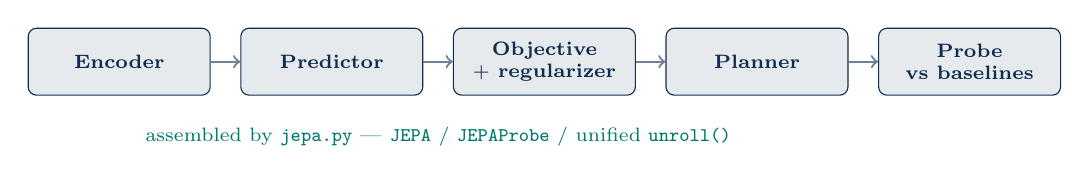
\begin{tikzpicture}[
      nd/.style={draw=primary, fill=primary!10, rounded corners=3pt, text width=2.1cm,
                 minimum height=0.85cm, align=center, font=\scriptsize\bfseries, text=primary, inner sep=3pt},
      ar/.style={->, thick, color=primary!60}]
      \node[nd] (a) at (0,0)    {Encoder};
      \node[nd] (b) at (2.7,0)  {Predictor};
      \node[nd] (c) at (5.4,0)  {Objective\\\scriptsize $+$ regularizer};
      \node[nd] (d) at (8.1,0)  {Planner};
      \node[nd] (e) at (10.8,0) {Probe\\\scriptsize vs baselines};
      \draw[ar](a)--(b); \draw[ar](b)--(c); \draw[ar](c)--(d); \draw[ar](d)--(e);
      \node[font=\scriptsize, text=secondary!80!black] at (4.05,-0.95)
        {assembled by \texttt{jepa.py} — \texttt{JEPA} / \texttt{JEPAProbe} / unified \texttt{unroll()}};
    \end{tikzpicture}}
  \end{center}
  \vspace{0.15cm}
  \begin{columns}[T]
    \begin{column}{0.5\textwidth}
      \begin{qbox}{secondary}{orgrow}
        \cardtitle{secondary}{Core engine — \texttt{eb\_jepa/} (swap these)}
        \footnotesize
        \qitem{\texttt{jepa.py} — \texttt{JEPA}/\texttt{JEPAProbe}, unified \texttt{unroll()}}
        \qitem{\texttt{architectures.py} — encoders / predictors (ResNet, Impala, GRU)}
        \qitem{\texttt{losses.py} — predictive JEPA \& anti-collapse (VICReg / VC / IDM)}
        \qitem{\texttt{planning.py} — CEM \,/\, MPPI planners \& objectives}
      \end{qbox}
    \end{column}
    \begin{column}{0.5\textwidth}
      \begin{qbox}{primary}{orgrow}
        \cardtitle{primary}{Around it — data \& assembly}
        \footnotesize
        \qitem{\texttt{datasets/<env>/} — loaders, dispatched by \texttt{env\_name}}
        \qitem{\texttt{examples/<x>/} — thin scripts: \texttt{main.py} · \texttt{eval.py} · \texttt{config.yaml} · README}
        \qitem{\texttt{launch\_sbatch.py} — one launcher (\texttt{--example}, submitit)}
        \qitem{\texttt{tests/} lock the swappable-module contracts}
      \end{qbox}
    \end{column}
  \end{columns}
  \vspace{0.1cm}
  \begin{center}\scriptsize\itshape Everything config-driven (\texttt{config.yaml} $+$ OmegaConf $+$ fire CLI) — change behaviour without touching the engine.\end{center}
\end{frame}

\begin{frame}{Pipeline — examples to reuse, tracks to complete, and above all: explore}
  \begin{center}\small\itshape Reuse a complete example, complete a track baseline by filling a tiny \texttt{\#TODO} surface — then explore.\end{center}
  \vspace{0.18cm}
  \begin{columns}[T]
    \begin{column}{0.5\textwidth}
      \begin{qbox}{secondary}{exrow}
        \cardtitle{secondary}{Reuse — complete examples}
        \footnotesize
        \qitem{\texttt{image\_jepa} — CIFAR-10 SSL, linear probe $\sim$91\%}
        \qitem{\texttt{video\_jepa} — Moving-MNIST latent prediction}
        \qitem{\texttt{ac\_video\_jepa/two\_rooms} — world model $+$ planning ($\sim$97\%)}
        \qitem{\itshape explore: \textbf{the maze} — A\textsuperscript{*}-free hierarchical navigation}
      \end{qbox}
    \end{column}
    \begin{column}{0.5\textwidth}
      \begin{qbox}{primary}{exrow}
        \cardtitle{primary}{Complete — 6 tracks (baseline $+$ \texttt{\#TODO})}
        \footnotesize
        \qitem{audio · EEG · point cloud · FinTime · LTSF · Gray-Scott}
        \qitem{\textbf{provided \& runnable}: loader $+$ augment $+$ train loop $+$ probe harness}
        \qitem{\textbf{you fill 3 \texttt{\#TODO} stubs}: \texttt{build\_encoder} · \texttt{build\_ssl}/\texttt{build\_jepa} · \texttt{probe}}
        \qitem{data side is config-only: \texttt{task\_type}/\texttt{in\_channels}/\texttt{metric} preset in \texttt{data\_config.yaml}}
      \end{qbox}
    \end{column}
  \end{columns}
  \vspace{0.12cm}
  \begin{center}\small\itshape ``Start from a baseline, then make it yours'': runnable harness $\rightarrow$ fill the stubs $\rightarrow$ your baseline $\rightarrow$ explore.\end{center}
\end{frame}

\begin{frame}{What We Expect From You}
  \vspace{0.2cm}
  \begin{center}
    \footnotesize\textbf{\color{primary}Start from a baseline example, then make it yours.}
  \end{center}
  \vspace{0.1cm}

  \begin{columns}[T]
    % --- Colonne de Gauche : Les Livrables ---
    \begin{column}{0.52\textwidth}
      \begin{qbox}{primary}{left1}
        \cardhead{primary}{01}{A working model}
        \footnotesize
        Train a JEPA world model on the data of your choice.\par\vspace{3pt}
        \qitem{Keep it reproducible (\texttt{config.yaml})}
        \qitem{Save at least one stable checkpoint}
      \end{qbox}
      
      \vspace{0.1cm}
      
      \begin{qbox}{primary}{left2}
        \cardhead{primary}{02}{10-minute presentation}
        \footnotesize
        Walk us through your approach, experiments, and findings.\par\vspace{3pt}
        \qitem{Explain your architectural choices}
        \qitem{Show what the model learned}
      \end{qbox}
    \end{column}

    % --- Colonne de Droite : Le Gold Standard ---
    \begin{column}{0.44\textwidth}
      \begin{qbox}{secondary}{right1}
        \cardtitle{secondary}{The Gold Standard}
        \vspace{0.1cm}
        \footnotesize
        \textit{What makes a great submission?}
        \par\vspace{0.3cm}
        
        \qitem{\textbf{Clear problem framing}}
        \qitem{\textbf{Quantitative results} vs. baseline}
        \qitem{\textbf{A genuine insight} or finding}
        \qitem{\textbf{Honest discussion} of limits}
        \qitem{\textbf{At least one ablation} study}

        \vspace{0.5cm}
        \centering
        
\begin{tikzpicture}
          \draw[secondary, thick, dashed] (0,0) circle (0.5cm);
          \node at (0,0) {\color{secondary}\Large\checkmark};
        \end{tikzpicture}
      \end{qbox}
    \end{column}
  \end{columns}
 \end{frame}
% =================================================================
% SECTION 2 — PRESENTATION REQUIREMENTS (les attendus)
% =================================================================
\section{Presentation Requirements}

\begin{frame}{What Your Presentation Should Cover}
  \begin{center}
    \vspace{0.4cm}
    \large Your 10-minute presentation should address the points below.\\[0.5cm]
    \small
    \textbf{Data} $\rightarrow$ \textbf{Architecture} $\rightarrow$
    \textbf{Training} $\rightarrow$ \textbf{Inference} $\rightarrow$
    \textbf{Evaluation} \\[0.2cm]
    (plus optional \textbf{Bonuses} to go further)
  \end{center}
\end{frame}

% --- Data ---
\begin{frame}{Data}
  \begin{center}
    \small\itshape Explain the data you trained on.
  \end{center}
  \vspace{0.35cm}
 
  \begin{columns}[T]
    % Q1
    \begin{column}{0.32\textwidth}
      \begin{qbox}{primary}{drow}
        \cardhead{secondary}{1}{Where is it from?}
        \footnotesize
        \qitem{\textbf{Generated} by you}
        \qitem{\textbf{Chosen} from the provided datasets}
        \qitem{\textbf{Found elsewhere} \, (cite the source)}
        \vspace{2pt}
        {\itshape\color{primary!70} Modality, size, difficulty?}
      \end{qbox}
    \end{column}
 
    % Q2
    \begin{column}{0.34\textwidth}
      \begin{qbox}{secondary}{drow}
        \cardhead{secondary}{2}{What does it look like?}
        \footnotesize Show it — stats, samples, a projection (PCA):
        \begin{center}
          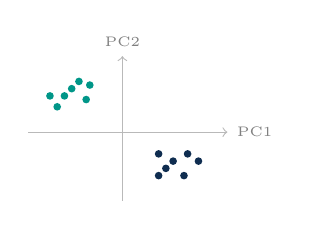
\begin{tikzpicture}[scale=0.92]
            \draw[->, gray!55] (-1.3,0) -- (1.45,0) node[right,font=\tiny,text=gray]{PC1};
            \draw[->, gray!55] (0,-0.95) -- (0,1.05) node[above,font=\tiny,text=gray]{PC2};
            \foreach \x/\y in {-0.8/0.5,-0.6/0.7,-0.9/0.35,-0.5/0.45,-0.7/0.6,-1.0/0.5,-0.45/0.65}
              \fill[secondary] (\x,\y) circle (1.5pt);
            \foreach \x/\y in {0.7/-0.4,0.5/-0.6,0.9/-0.3,0.6/-0.5,0.85/-0.6,1.05/-0.4,0.5/-0.3}
              \fill[primary] (\x,\y) circle (1.5pt);
          \end{tikzpicture}
        \end{center}
      \end{qbox}
    \end{column}
 
    % Q3
    \begin{column}{0.32\textwidth}
      \begin{qbox}{primary}{drow}
        \cardhead{secondary}{3}{How did you prepare it?}
        \footnotesize
        \qitem{Normalisation}
        \qitem{Encoding / decoding target}
        \qitem{Data augmentation?}
        \vspace{2pt}
        {\itshape\color{primary!70} Any preprocessing worth noting?}
      \end{qbox}
    \end{column}
  \end{columns}
\end{frame}
 
% --- Architecture ---
\begin{frame}{Architecture}
  \begin{center}
    \small\itshape Describe your model and how it was trained.
  \end{center}
  \vspace{0.35cm}
 
  \begin{columns}[T]
    % Model card
    \begin{column}{0.46\textwidth}
      \begin{qbox}{primary}{arow}
        \cardtitle{primary}{The model}
        \footnotesize
        \qitem{\textbf{Unchanged?} \, A quick JEPA recap}
        \qitem{\textbf{Modified?} \, Why, what, intuition, papers}
        \qitem{Number of parameters \& modules}
      \end{qbox}
    \end{column}
 
    % Loss / dynamics card
    \begin{column}{0.52\textwidth}
      \begin{qbox}{secondary}{arow}
        \cardtitle{secondary}{Loss \& training dynamics}
        \footnotesize
        \begin{columns}[c]
          \begin{column}{0.62\textwidth}
            \qitem{Which (sub)losses? how balanced?}
            \qitem{Representation collapse — observed?}
            \qitem{Regularisation \& stability}
          \end{column}
          \begin{column}{0.36\textwidth}
            \centering
            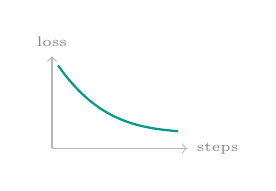
\begin{tikzpicture}[scale=0.78]
              \draw[->, gray!55] (0,0) -- (2.2,0) node[right,font=\tiny,text=gray]{steps};
              \draw[->, gray!55] (0,0) -- (0,1.5) node[above,font=\tiny,text=gray]{loss};
              \draw[secondary, thick] (0.1,1.35) .. controls (0.7,0.5) and (1.3,0.34) .. (2.05,0.28);
            \end{tikzpicture}\\[-2pt]
            {\scriptsize\itshape training curve}
          \end{column}
        \end{columns}
      \end{qbox}
    \end{column}
  \end{columns}
\end{frame}

% --- Training ---
\begin{frame}{Training}
  \begin{center}
    \small\itshape How did you train, and how did you iterate efficiently?
  \end{center}
  \vspace{0.35cm}

  \begin{columns}[T]
    % Setup card
    \begin{column}{0.46\textwidth}
      \begin{qbox}{primary}{trow}
        \cardtitle{primary}{Setup}
        \footnotesize
        \qitem{Batch size, optimiser}
        \qitem{Learning-rate scheduler}
        \qitem{Number of epochs}
      \end{qbox}
    \end{column}

    % Comparing card
    \begin{column}{0.52\textwidth}
      \begin{qbox}{secondary}{trow}
        \cardtitle{secondary}{Comparing without full training}
        \footnotesize
        \qitem{A \textbf{proxy metric} to rank runs early}
        \qitem{A strategy to compare \emph{without} a full run}
        \vspace{2pt}
        {\itshape\color{primary!70} e.g.\ scaling laws, ablations, \ldots}
      \end{qbox}
    \end{column}
  \end{columns}
\end{frame}

% --- Inference ---
\begin{frame}{Inference}
  \begin{center}
    \small\itshape How do you use the trained model?
  \end{center}
  \vspace{0.35cm}

  \begin{columns}[T]
    \begin{column}{0.52\textwidth}
      \begin{qbox}{primary}{irow}
        \cardtitle{primary}{Inference strategy}
        \footnotesize
        \qitem{Method $\rightarrow$ Mode 1 / Mode 2, MCTS, actor, \ldots?}
        \qitem{Performance vs.\ inference time}
        \qitem{Any inference tricks?}
      \end{qbox}
    \end{column}
    \begin{column}{0.44\textwidth}
      \begin{qbox}{secondary}{irow}
        \cardtitle{secondary}{Performance vs.\ time}
        \centering
        \begin{tikzpicture}[scale=0.82]
          \draw[->, gray!55] (0,0) -- (2.3,0) node[right,font=\tiny,text=gray]{time};
          \draw[->, gray!55] (0,0) -- (0,1.5) node[above,font=\tiny,text=gray]{perf.};
          \draw[secondary, thick] (0.1,0.25) .. controls (0.8,1.0) and (1.4,1.2) .. (2.2,1.3);
        \end{tikzpicture}\\[-2pt]
        {\footnotesize\itshape more compute, better rollout?}
      \end{qbox}
    \end{column}
  \end{columns}
\end{frame}

% --- Evaluation ---
\begin{frame}{Evaluation}
  \begin{center}
    \small\itshape How good is it, and how do you know?
  \end{center}
  \vspace{0.35cm}

  \begin{columns}[T]
    \begin{column}{0.32\textwidth}
      \begin{qbox}{primary}{erow}
        \cardtitle{primary}{Robustness}
        \footnotesize
        \qitem{Ablations}
        \qitem{Scaling laws}
        \qitem{Seed \& training stability}
      \end{qbox}
    \end{column}
    \begin{column}{0.32\textwidth}
      \begin{qbox}{secondary}{erow}
        \cardtitle{secondary}{Performance}
        \footnotesize
        \qitem{Dataset performance}
        \qitem{Compare to a baseline}
      \end{qbox}
    \end{column}
    \begin{column}{0.32\textwidth}
      \begin{qbox}{primary}{erow}
        \cardtitle{primary}{Reach}
        \footnotesize
        \qitem{Application to real-life situations}
        \qitem{A step towards AGI?}
      \end{qbox}
    \end{column}
  \end{columns}
\end{frame}

% --- Bonuses ---
\begin{frame}{Bonuses}
  \begin{center}
    \small\itshape Optional — ways to stand out.
  \end{center}
  \vspace{0.35cm}

  \begin{columns}[T]
    \begin{column}{0.48\textwidth}
      \begin{qbox}{primary}{brow}
        \cardtitle{primary}{Rewarded}
        \footnotesize
        \qitem{High performance}
        \qitem{Hyperparameter tuning}
        \qitem{Extensive training-stability analysis — esp.\ visualising representation collapse}
      \end{qbox}
    \end{column}
    \begin{column}{0.48\textwidth}
      \begin{qbox}{secondary}{brow}
        \cardtitle{secondary}{Going further}
        \footnotesize
        \qitem{Handmade (non-synthetic) dataset}
        \qitem{Method that scales to other datasets of the field (e.g.\ time series)}
        \qitem{Hierarchical world models}
      \end{qbox}
    \end{column}
  \end{columns}
\end{frame}

% =================================================================
% SECTION 3 — THE MAZE EXAMPLE  (left blank for now)
% =================================================================
\section{The Maze Example}

\begin{frame}{The Maze Example}
  % TODO: à compléter
\end{frame}

% =================================================================
% LOGISTICS — Timeline & Judging
% =================================================================
\section{Timeline \& Judging}
\begin{frame}{Timeline \& Judging}
  \vspace{0.35cm}
  \begin{columns}[T]

    % --- Colonne 1 : Timeline ---
    \begin{column}{0.48\textwidth}
      \begin{qbox}{primary}{sched}
        \cardtitle{primary}{Schedule}
        \footnotesize
        \begin{description}[\hspace{1.3cm}]
          \item[\textcolor{secondary}{17:30}] Code submission
          \vspace{0.2cm}
          \item[\textcolor{secondary}{18:00}] Slides submission \& pre-jury
          \vspace{0.2cm}
          \item[\textcolor{secondary}{19:00}] Final jury \textit{(qualified teams)}
        \end{description}
        
        \vspace{0.7cm}
        \centering
        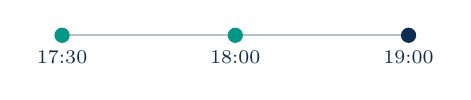
\begin{tikzpicture}[scale=1.1]
          \draw[thick, primary!30] (0,0) -- (4,0);
          \fill[secondary] (0,0) circle (2.5pt) node[below, text=primary, font=\scriptsize, yshift=-2pt] {17:30};
          \fill[secondary] (2,0) circle (2.5pt) node[below, text=primary, font=\scriptsize, yshift=-2pt] {18:00};
          \fill[primary]   (4,0) circle (2.5pt) node[below, text=primary, font=\scriptsize, yshift=-2pt] {19:00};
        \end{tikzpicture}
        \vspace{0.1cm}
      \end{qbox}
    \end{column}

    % --- Colonne 2 : Judging ---
    \begin{column}{0.48\textwidth}
      \begin{qbox}{secondary}{sched}
        \cardtitle{secondary}{Judging Criteria}
        \footnotesize
        \vspace{0.15cm}
        
        \qitem{\textbf{Technical quality}\\ \textit{\color{black!60}Robustness, code cleanliness \& architecture}}
        \vspace{0.15cm}
        
        \qitem{\textbf{Results}\\ \textit{\color{black!60}Performance, metrics \& meaningful comparisons}}
        \vspace{0.15cm}
        
        \qitem{\textbf{Presentation}\\ \textit{\color{black!60}Clarity, storytelling \& visual aids}}
        \vspace{0.15cm}
        
        \qitem{\textbf{Originality}\\ \textit{\color{black!60}Ablations, novel insights \& going the extra mile}}

      \end{qbox}
    \end{column}

  \end{columns}
\end{frame}

% ---------------------------------------------------------------
% CLOSING
% ---------------------------------------------------------------
\begin{frame}{ }
  \begin{center}
    \vspace{1cm}
    {\color{primary}\Huge\bfseries Now go build your world.}\\[1cm]
    {\large\color{secondary}\itshape Good luck, and have fun!}
  \end{center}
\end{frame}

\end{document}
